% Template adapted from https://github.com/jgm/pandoc-templates/blob/master/default.latex
% To be used with XeLaTex in memoiR
%%%%%%%%%%%%%%%%%%%%%%%%%%%%%%%%%%%%%%%%%%%%%%%%%%%%%%%%%%%%%%%%%%%%%%%%%%%%%%%%%%%%%%%%%

% Options for packages loaded elsewhere
\PassOptionsToPackage{unicode=true}{hyperref}
\PassOptionsToPackage{hyphens}{url}
\PassOptionsToPackage{dvipsnames,svgnames*,x11names*}{xcolor}
% Right to left support


\documentclass[
  10pt,
  italian,
  a4paper,
  extrafontsizes,onecolumn,openright
  ]{memoir}

% Double (or whatever) spacing

% Math
\usepackage{amssymb, amsmath}
% mathspec: arbitrary math fonts
\usepackage{unicode-math}
\defaultfontfeatures{Scale=MatchLowercase}
\defaultfontfeatures[\rmfamily]{Ligatures=TeX,Scale=1}

% Fonts
\usepackage{lmodern}
\usepackage{fontspec}

% Main font
% Specific sanserif font
% Specific monotype font
\setmonofont[Scale=0.75]{Operator Mono SSm Lig Book}
% Specific math font
% Chinese, Japanese, Corean fonts

% Use upquote for straight quotes in verbatim environments
\usepackage{upquote}
% Use microtype
\usepackage[]{microtype}
\UseMicrotypeSet[protrusion]{basicmath} % disable protrusion for tt fonts

% Verbatim in note

% Color links
\usepackage{xcolor}

% Strikeout

% Necessary for code chunks
\usepackage{color}
\usepackage{fancyvrb}
\newcommand{\VerbBar}{|}
\newcommand{\VERB}{\Verb[commandchars=\\\{\}]}
\DefineVerbatimEnvironment{Highlighting}{Verbatim}{commandchars=\\\{\}}
% Add ',fontsize=\small' for more characters per line
\usepackage{framed}
\definecolor{shadecolor}{RGB}{248,248,248}
\newenvironment{Shaded}{\begin{snugshade}}{\end{snugshade}}
\newcommand{\AlertTok}[1]{\textcolor[rgb]{0.94,0.16,0.16}{#1}}
\newcommand{\AnnotationTok}[1]{\textcolor[rgb]{0.56,0.35,0.01}{\textbf{\textit{#1}}}}
\newcommand{\AttributeTok}[1]{\textcolor[rgb]{0.77,0.63,0.00}{#1}}
\newcommand{\BaseNTok}[1]{\textcolor[rgb]{0.00,0.00,0.81}{#1}}
\newcommand{\BuiltInTok}[1]{#1}
\newcommand{\CharTok}[1]{\textcolor[rgb]{0.31,0.60,0.02}{#1}}
\newcommand{\CommentTok}[1]{\textcolor[rgb]{0.56,0.35,0.01}{\textit{#1}}}
\newcommand{\CommentVarTok}[1]{\textcolor[rgb]{0.56,0.35,0.01}{\textbf{\textit{#1}}}}
\newcommand{\ConstantTok}[1]{\textcolor[rgb]{0.00,0.00,0.00}{#1}}
\newcommand{\ControlFlowTok}[1]{\textcolor[rgb]{0.13,0.29,0.53}{\textbf{#1}}}
\newcommand{\DataTypeTok}[1]{\textcolor[rgb]{0.13,0.29,0.53}{#1}}
\newcommand{\DecValTok}[1]{\textcolor[rgb]{0.00,0.00,0.81}{#1}}
\newcommand{\DocumentationTok}[1]{\textcolor[rgb]{0.56,0.35,0.01}{\textbf{\textit{#1}}}}
\newcommand{\ErrorTok}[1]{\textcolor[rgb]{0.64,0.00,0.00}{\textbf{#1}}}
\newcommand{\ExtensionTok}[1]{#1}
\newcommand{\FloatTok}[1]{\textcolor[rgb]{0.00,0.00,0.81}{#1}}
\newcommand{\FunctionTok}[1]{\textcolor[rgb]{0.00,0.00,0.00}{#1}}
\newcommand{\ImportTok}[1]{#1}
\newcommand{\InformationTok}[1]{\textcolor[rgb]{0.56,0.35,0.01}{\textbf{\textit{#1}}}}
\newcommand{\KeywordTok}[1]{\textcolor[rgb]{0.13,0.29,0.53}{\textbf{#1}}}
\newcommand{\NormalTok}[1]{#1}
\newcommand{\OperatorTok}[1]{\textcolor[rgb]{0.81,0.36,0.00}{\textbf{#1}}}
\newcommand{\OtherTok}[1]{\textcolor[rgb]{0.56,0.35,0.01}{#1}}
\newcommand{\PreprocessorTok}[1]{\textcolor[rgb]{0.56,0.35,0.01}{\textit{#1}}}
\newcommand{\RegionMarkerTok}[1]{#1}
\newcommand{\SpecialCharTok}[1]{\textcolor[rgb]{0.00,0.00,0.00}{#1}}
\newcommand{\SpecialStringTok}[1]{\textcolor[rgb]{0.31,0.60,0.02}{#1}}
\newcommand{\StringTok}[1]{\textcolor[rgb]{0.31,0.60,0.02}{#1}}
\newcommand{\VariableTok}[1]{\textcolor[rgb]{0.00,0.00,0.00}{#1}}
\newcommand{\VerbatimStringTok}[1]{\textcolor[rgb]{0.31,0.60,0.02}{#1}}
\newcommand{\WarningTok}[1]{\textcolor[rgb]{0.56,0.35,0.01}{\textbf{\textit{#1}}}}

% Listings package

% Tables
\usepackage{longtable,booktabs,tabu}
% Fix footnotes in tables (requires footnote package)
\IfFileExists{footnote.sty}{\usepackage{footnote}\makesavenoteenv{longtable}}{}

% Graphics
\usepackage{graphicx,grffile}
\graphicspath{{images/}}
\makeatletter
\def\maxwidth{\ifdim\Gin@nat@width>\linewidth\linewidth\else\Gin@nat@width\fi}
\def\maxheight{\ifdim\Gin@nat@height>\textheight\textheight\else\Gin@nat@height\fi}
\makeatother
% Scale images if necessary, so that they will not overflow the page
% margins by default, and it is still possible to overwrite the defaults
% using explicit options in \includegraphics[width, height, ...]{}
\setkeys{Gin}{width=\maxwidth,height=\maxheight,keepaspectratio}

% Prevent overfull lines
\setlength{\emergencystretch}{3em}  
\providecommand{\tightlist}{%
  \setlength{\itemsep}{0pt}\setlength{\parskip}{0pt}}

% Number sections for memoir (secnumdepth counter is ignored)
\setsecnumdepth{section}

% Set default figure placement to htbp
\makeatletter
\def\fps@figure{htbp}
\makeatother

% Spacing in lists
\usepackage{enumitem}

% Polyglossia
\usepackage{polyglossia}
\setmainlanguage{it}
\setotherlanguage{en-US}

% BibLaTeX
\usepackage[backend=biber,style=authoryear-ibid,isbn=false,backref=true,giveninits=true,uniquename=init,maxcitenames=2,maxbibnames=150,sorting=nyt,sortcites=false,style=apa]{biblatex}
\addbibresource{refs.bib}

% cslreferences environment required by pandoc > 2.7



%%%%%%%%%%%%%%%%%%%%%%%%%%%%%%%%%%%%%%%%%%%%%%%%%%%%%%%%%%
% memoiR format

% Chapter Summary environment 
\usepackage[tikz]{bclogo}
\newenvironment{Summary}
  {\begin{bclogo}[logo=\bctrombone, noborder=true, couleur=lightgray!50]{In breve}\parindent0pt}
  {\end{bclogo}}
% Syntax:
%
%```{block, type='Summary'}
% Deliver message here.
% ```

% scriptsize code 
\let\oldverbatim\verbatim
\def\verbatim{\oldverbatim\scriptsize}
% Applies to code blocks and R code results
% code chunk options size='scriptsize' applies only to R code and results
% if the code chunk sets a different size, \def\verbatim{...} is prioritary for code results 


% Layout
%%%%%%%%%%%%%%%%%%%%%%%%%%%%%%%%%%%%%%%%%%%%%%%%%%%%%%%%%%

% Based on memoir, style companion
\newcommand{\MemoirChapStyle}{daleif1}
\newcommand{\MemoirPageStyle}{Ruled}

% Space between paragraphs
\usepackage{parskip}
  \abnormalparskip{3pt}

% Adjust margin paragraphs vertical position
\usepackage{marginfix}


% Margins
%%%%%%%%%%%%%%%%%%%%%%%%%%%%%%%%%%%%%%%

% allow use of '-',+','/' ans '*' to make simple length computation
\usepackage{calc}

% Full-width figures utilities
\newlength\widthw % full width
\newlength{\rf}
\newcommand*{\definesHSpace}{
  \strictpagecheck % slower but efficient detection of odd/even pages
  \checkoddpage
  \ifoddpage
  \setlength{\rf}{0mm}
  \else
  \setlength{\rf}{\marginparsep+\marginparwidth}
  \fi
}

\makeatletter
% 1" margins for the front matter.
\newcommand*{\SmallMargins}{
  \setlrmarginsandblock{1.5in}{1.5in}{*}
  \setmarginnotes{0.1in}{0.1in}{0.1in}
 \setulmarginsandblock{1.5in}{1in}{*}
  \checkandfixthelayout
  \ch@ngetext
  \clearpage
  \setlength{\widthw}{\textwidth+\marginparsep+\marginparwidth}
  \footnotesatfoot
  \chapterstyle{\MemoirChapStyle}  % Chapter and page styles must be recalled
  \pagestyle{\MemoirPageStyle}
}

% 3" outer margin for the main matter
\newcommand{\LargeMargins}{\SmallMargins}
\makeatother

% Figure captions and footnotes in outer margins


% Main title page with filigrane
%%%%%%%%%%%%%%%%%%%%%%%%%%%%%%%%%%%%%%%%%%%%%%%%%%%%%%%%%%

% Text blocks
\usepackage[absolute,overlay]{textpos}
  \setlength{\TPHorizModule}{1mm}
  \setlength{\TPVertModule}{1mm}

\newcommand{\MainTitlePage}[2]{
  \SmallMargins % Margins
  \pagestyle{empty} % No header/footer
  \textblockorigin{\stockwidth-\paperwidth-\trimedge}{\trimtop} % recto
  \begin{textblock*}{2mm}(\spinemargin/2,\uppermargin/2)
    \rule{1pt}{\paperheight-\uppermargin}
  \end{textblock*}
  \begin{textblock*}{\paperwidth*2/3}(\paperwidth/5, \paperheight/5)
    \flushright
    \begin{Spacing}{3}
      {\fontfamily{qtm}\selectfont\fontsize{45}{45}\selectfont\textsc{\thetitle}}
    \end{Spacing}
  \end{textblock*}
    \begin{textblock*}{\paperwidth*2/3}(\paperwidth/5, \paperheight/2)
    \flushright
    {\fontfamily{qtm}\huge\theauthor}
  \end{textblock*}
    \begin{textblock*}{\paperwidth*2/3}[0, 1](\spinemargin, \uppermargin+\textheight)
    \normalfont\thedate
  \end{textblock*}
  ~\\ % Print a character or the page will not exist
  \newpage
  \textblockorigin{\trimedge}{\trimtop} % verso
  \begin{textblock*}{\textwidth}(\paperwidth-\spinemargin-\textwidth, \uppermargin)
    #1
  \end{textblock*}
  \begin{textblock*}{\textwidth}[0,1](\paperwidth-\spinemargin-\textwidth, \uppermargin+\textheight+\footskip)
    \centering
    
\includegraphics[width=\paperwidth/4]{logo}\\ \bigskip
    #2
  \end{textblock*}
  ~\\ % Print a character or the page will not exist
  \newpage
}

% Clear page and open an even one (\clearpage opens an odd one)
\newcommand{\evenpage}{
  \clearpage
  \strictpagecheck % slower but efficient detection of odd/even pages
  \checkoddpage
  \ifoddpage
    \thispagestyle{empty}
    ~\\ % Print a character or the page will not exist
    \newpage
  \else
    % do nothing
  \fi
}


%% PDF title page to insert
%%%%%%%%%%%%%%%%%%%%%%%%%%%%%%%%%%%%%%%%%%%%%%%%%%%%%%%%%%



%% Bibliography
%%%%%%%%%%%%%%%%%%%%%%%%%%%%%%%%%%%%%%%%%%%%%%%%%%%%%%%%%%

\usepackage[strict,autostyle]{csquotes}
% Repeated citation as author-year-title instead of author-title (modification of footcite:note in verbose-inote.cbx)

%% Table of Contents
%%%%%%%%%%%%%%%%%%%%%%%%%%%%%%%%%%%%%%%%%%%%%%%%%%%%%%%%%%

% fix the typesetting of the part number
\renewcommand\partnumberlinebox[2]{#2\ ---\ }


% Fonts
%%%%%%%%%%%%%%%%%%%%%%%%%%%%%%%%%%%%%%%%%%%%%%%%%%%%%%%%%%


% Hyperref comes last
%%%%%%%%%%%%%%%%%%%%%%%%%%%%%%%%%%%%%%%%%%%%%%%%%%%%%%%%%%

\usepackage{hyperref}
\hypersetup{
  pdftitle={Psicometria},
  pdfauthor={Corrado Caudek},
  colorlinks=true,
  linkcolor=Maroon,
  citecolor=Blue,
  urlcolor=Blue,
  breaklinks=true}

% Don't use monospace font for urls
\urlstyle{same}


% Title, author, date from YAML to LaTeX
%%%%%%%%%%%%%%%%%%%%%%%%%%%%%%%%%%%%%%%%%%%%%%%%%%%%%%%%%%

\title{Psicometria}

\author{Corrado Caudek}

\date{2021-12-14}


% Include headers (preamble.tex) here
%%%%%%%%%%%%%%%%%%%%%%%%%%%%%%%%%%%%%%%%%%%%%%%%%%%%%%%%%%
% Add LaTeX code into the preamble of the document here
\hyphenation{bio-di-ver-si-ty sap-lings}


%%%%%%%%%%%%%%%%%%%%%%%%%%%%%%%%%%%%%%%%%%%%%%%%%%%%%%%%%%%%%%%%%%%%%%%%%
% memoiR dalef3 chapter style 
% https://ctan.crest.fr/tex-archive/info/latex-samples/MemoirChapStyles/MemoirChapStyles.pdf
\usepackage{soul}
\definecolor{nicered}{rgb}{.647,.129,.149}
\makeatletter
\newlength\dlf@normtxtw
\setlength\dlf@normtxtw{\textwidth}
\def\myhelvetfont{\def\sfdefault{mdput}}
\newsavebox{\feline@chapter}
\newcommand\feline@chapter@marker[1][4cm]{%
  \sbox\feline@chapter{%
    \resizebox{!}{#1}{\fboxsep=1pt%
	  \colorbox{nicered}{\color{white}\bfseries\sffamily\thechapter}%
	}}%
  \rotatebox{90}{%
    \resizebox{%
	  \heightof{\usebox{\feline@chapter}}+\depthof{\usebox{\feline@chapter}}}%
	{!}{\scshape\so\@chapapp}}\quad%
  \raisebox{\depthof{\usebox{\feline@chapter}}}{\usebox{\feline@chapter}}%
 }
\newcommand\feline@chm[1][4cm]{%
  \sbox\feline@chapter{\feline@chapter@marker[#1]}%
  \makebox[0pt][l]{% aka \rlap
    \makebox[1cm][r]{\usebox\feline@chapter}%
  }}
\makechapterstyle{daleif1}{
  \renewcommand\chapnamefont{\normalfont\Large\scshape\raggedleft\so}
  \renewcommand\chaptitlefont{\normalfont\huge\bfseries\scshape\color{nicered}}
  \renewcommand\chapternamenum{}
  \renewcommand\printchaptername{}
  \renewcommand\printchapternum{\null\hfill\feline@chm[2.5cm]\par}
  \renewcommand\afterchapternum{\par\vskip\midchapskip}
  \renewcommand\printchaptertitle[1]{\chaptitlefont\raggedleft ##1\par}
}
\makeatother

\DeclareMathOperator{\Var}{Var} % Define variance operator
\DeclareMathOperator{\SD}{SD} % Define sd operator
\DeclareMathOperator{\Cov}{Cov} % Define covariance operator
\DeclareMathOperator{\Corr}{Corr} % Define correlation operator
\DeclareMathOperator{\Me}{Me} % Define mediane operator
\DeclareMathOperator{\Mo}{Mo} % Define mode operator
\DeclareMathOperator{\Bin}{Bin} % Define binomial operator
\DeclareMathOperator{\Bernoulli}{Bernoulli} % Define Bernoulli operator
\DeclareMathOperator{\Poi}{Poi} % Define Poisson operator
\DeclareMathOperator{\Uniform}{Uniform} % Define Uniform operator
\DeclareMathOperator{\Cauchy}{Cauchy} % Define Cauchy operator
\DeclareMathOperator{\elpd}{elpd} % Define elpd operator
\DeclareMathOperator{\lppd}{lppd} % Define lppd operator
\DeclareMathOperator{\LOO}{LOO} % Define LOO operator
\DeclareMathOperator{\B}{\mathscr{B}} % Define Bernoulli operator
\newcommand{\R}{\textsf{R}} % Define R programming language symbol
\newcommand{\E}{\mathbb{E}} % Define expected value operator
\newcommand{\Real}{\mathbb{R}} % Define real number operator
\newcommand{\Prob}{\mathscr{P}}
\DeclareMathOperator*{\argmin}{arg\,min} % thin space, limits on side in displays
\DeclareMathOperator*{\argmax}{arg\,max} % thin space, limits on side in displays

\raggedbottom % allow variable (ragged) site heights
\frenchspacing

\usepackage[
  labelfont=bf, 
  font={small, it} 
]{caption} 
\usepackage{upquote} % print correct quotes in verbatim-environments
\usepackage{empheq} 
\usepackage{xfrac}
\usepackage{lstbayes}




\usepackage{booktabs}
\usepackage{longtable}
\usepackage{array}
\usepackage{multirow}
\usepackage{wrapfig}
\usepackage{float}
\usepackage{colortbl}
\usepackage{pdflscape}
\usepackage{tabu}
\usepackage{threeparttable}
\usepackage{threeparttablex}
\usepackage[normalem]{ulem}
\usepackage{makecell}
\usepackage{xcolor}


% End of preamble
%%%%%%%%%%%%%%%%%%%%%%%%%%%%%%%%%%%%%%%%%%%%%%%%%%%%%%%%%%


\usepackage{amsthm}
\newtheorem{theorem}{Teorema}[chapter]
\newtheorem{lemma}{Lemma}[chapter]
\newtheorem{corollary}{Corollario}[chapter]
\newtheorem{proposition}{Proposizione}[chapter]
\newtheorem{conjecture}{Congettura}[chapter]
\theoremstyle{definition}
\newtheorem{definition}{Definizione}[chapter]
\theoremstyle{definition}
\newtheorem{example}{Esempio}[chapter]
\theoremstyle{definition}
\newtheorem{exercise}{Exercizio}[chapter]
\theoremstyle{definition}
\newtheorem{hypothesis}{Hypothesis}[chapter]
\theoremstyle{remark}
\newtheorem*{remark}{Osservazione}
\newtheorem*{solution}{Soluzione}
\begin{document}
\frontmatter

% Title page
%%%%%%%%%%%%%%%%%%%%%%%%%%%%%%%%%%%%%%%%%%%%%%%%%%%%%%%%%%


\MainTitlePage{Questo documento è stato realizzato con:

\begin{itemize}
  \item \LaTeX\; e la classe memoir (\url{http://www.ctan.org/pkg/memoir});
  \item $\R$ (\url{http://www.r-project.org/}) e RStudio (\url{http://www.rstudio.com/});
  \item bookdown (\url{http://bookdown.org/}) e memoiR (\url{https://ericmarcon.github.io/memoiR/}).
\end{itemize}}{Nel blog della mia pagina personale sono forniti alcuni approfondimenti degli argomenti qui trattati.

\url{https://ccaudek.github.io/caudeklab/}}


% Before Body
%%%%%%%%%%%%%%%%%%%%%%%%%%%%%%%%%%%%%%%%%%%%%%%%%%%%%%%%%%





% Contents
%%%%%%%%%%%%%%%%%%%%%%%%%%%%%%%%%%%%%%%%%%%%%%%%%%%%%%%%%%

\LargeMargins
{
\hypersetup{linkcolor=}
\setcounter{tocdepth}{2}
\tableofcontents
}


% Body
%%%%%%%%%%%%%%%%%%%%%%%%%%%%%%%%%%%%%%%%%%%%%%%%%%%%%%%%%%

\LargeMargins
\scriptsize

\normalsize

\chapter*{}

\vfill

\scriptsize

\normalsize

\scriptsize

Copyright \(\copyright\) 2022.

\normalsize

Data della versione presente: Dicembre 14, 2021.

\hypertarget{prefazione}{%
\chapter{Prefazione}\label{prefazione}}

\textbf{Data Science per psicologi} contiene il materiale delle lezioni dell'insegnamento di \emph{Psicometria B000286} (A.A. 2021/2022) rivolto agli studenti del primo anno del Corso di Laurea in Scienze e Tecniche Psicologiche dell'Università degli Studi di Firenze.

L'insegnamento di Psicometria si propone di fornire agli studenti un'introduzione all'analisi dei dati in psicologia.
Le conoscenze/competenze che verranno sviluppate in questo insegnamento sono quelle della \emph{Data science}, ovvero le conoscenze/competenze che si pongono all'intersezione tra statistica (ovvero, richiedono la capacità di comprendere teoremi statistici) e informatica (ovvero, richiedono la capacità di sapere utilizzare un software).

\hypertarget{la-psicologia-e-la-data-science}{%
\section*{La psicologia e la Data Science}\label{la-psicologia-e-la-data-science}}
\addcontentsline{toc}{section}{La psicologia e la Data Science}

\begin{quote}
It's worth noting, before getting started, that this material is hard. If you find yourself confused at any point, you are normal. Any sense of confusion you feel is just your brain correctly calibrating to the subject matter. Over time, confusion is replaced by comprehension {[}\ldots{]} --- Richard McElreath
\end{quote}

Sembra sensato spendere due parole su un tema che è importante per gli studenti: quello indicato dal titolo di questo Capitolo. È ovvio che agli studenti di psicologia la statistica non piace. Se piacesse, forse studierebbero Data Science e non psicologia; ma non lo fanno. Di conseguenza, gli studenti di psicologia si chiedono: ``perché dobbiamo perdere tanto tempo a studiare queste cose quando in realtà quello che ci interessa è tutt'altro?'\,' Questa è una bella domanda.

C'è una ragione molto semplice che dovrebbe farci capire perché la Data Science è così importante per la psicologia. Infatti, a ben pensarci, la psicologia è una disciplina intrinsecamente statistica, se per statistica intendiamo quella disciplina che studia la variazione delle caratteristiche degli individui nella popolazione. La psicologia studia \emph{gli individui} ed è proprio la variabilità inter- e intra-individuale ciò che vogliamo descrivere e, in certi casi, predire. In questo senso, la psicologia è molto diversa dall'ingegneria, per esempio. Le proprietà di un determinato ponte sotto certe condizioni, ad esempio, sono molto simili a quelle di un altro ponte, sotto le medesime condizioni. Quindi, per un ingegnere la statistica è poco importante: le proprietà dei materiali sono unicamente dipendenti dalla loro composizione e restano costanti. Ma lo stesso non può dirsi degli individui: ogni individuo è unico e cambia nel tempo. E le variazioni tra gli individui, e di un individuo nel tempo, sono l'oggetto di studio proprio della psicologia: è dunque chiaro che i problemi che la psicologia si pone sono molto diversi da quelli affrontati, per esempio, dagli ingegneri. Questa è la ragione per cui abbiamo tanto bisogno della \emph{data science} in psicologia: perché la \emph{data science} ci consente di descrivere la variazione e il cambiamento. E queste sono appunto le caratteristiche di base dei fenomeni psicologici.

Sono sicuro che, leggendo queste righe, a molti studenti sarà venuta in mente la seguente domanda: perché non chiediamo a qualche esperto di fare il ``lavoro sporco'' (ovvero le analisi statistiche) per noi, mentre noi (gli psicologi) ci occupiamo solo di ciò che ci interessa, ovvero dei problemi psicologici slegati dai dettagli ``tecnici'' della \emph{data science}?
La risposta a questa domanda è che non è possibile progettare uno studio psicologico sensato senza avere almeno una comprensione rudimentale della \emph{data science}. Le tematiche della \emph{data science} non possono essere ignorate né dai ricercatori in psicologia né da coloro che svolgono la professione di psicologo al di fuori dell'Università. Infatti, anche i professionisti al di fuori dall'università non possono fare a meno di leggere la letteratura psicologica più recente: il continuo aggiornamento delle conoscenze è infatti richiesto dalla deontologia della professione. Ma per potere fare questo è necessario conoscere un bel po' di \emph{data science}! Basta aprire a caso una rivista specialistica di psicologia per rendersi conto di quanto ciò sia vero: gli articoli che riportano i risultati delle ricerche psicologiche sono zeppi di analisi statistiche e di modelli formali. E la comprensione della letteratura psicologica rappresenta un requisito minimo nel bagaglio professionale dello psicologo.

Le considerazioni precedenti cercano di chiarire il seguente punto: la \emph{data science} non è qualcosa da studiare a malincuore, in un singolo insegnamento universitario, per poi poterla tranquillamente dimenticare. Nel bene e nel male, gli psicologi usano gli strumenti della \emph{data science} in tantissimi ambiti della loro attività professionale: in particolare quando costruiscono, somministrano e interpretano i test psicometrici. È dunque chiaro che possedere delle solide basi di \emph{data science} è un tassello imprescindibile del bagaglio professionale dello psicologo. In questo insegnamento verrano trattati i temi base della \emph{data science} e verrà adottato un punto di vista bayesiano, che corrisponde all'approccio più recente e sempre più diffuso in psicologia.

\hypertarget{come-studiare}{%
\section*{Come studiare}\label{come-studiare}}
\addcontentsline{toc}{section}{Come studiare}

\begin{quote}
I know quite certainly that I myself have no special talent. Curiosity, obsession and dogged endurance, combined with self-criticism, have brought me to my ideas. --- Albert Einstein
\end{quote}

Il giusto metodo di studio per prepararsi all'esame di Psicometria è quello di seguire attivamente le lezioni, assimilare i concetti via via che essi vengono presentati e verificare in autonomia le procedure presentate a lezione. Incoraggio gli studenti a farmi domande per chiarire ciò che non è stato capito appieno. Incoraggio gli studenti a utilizzare i forum attivi su Moodle e, soprattutto, a svolgere gli esercizi proposti su Moodle. I problemi forniti su Moodle rappresentano il livello di difficoltà richiesto per superare l'esame e consentono allo studente di comprendere se le competenze sviluppate fino a quel punto sono sufficienti rispetto alle richieste dell'esame.

La prima fase dello studio, che è sicuramente individuale, è quella in cui è necessario acquisire le conoscenze teoriche relative ai problemi che saranno presentati all'esame. La seconda fase di studio, che può essere facilitata da scambi con altri e da incontri di gruppo, porta ad acquisire la capacità di applicare le conoscenze: è necessario capire come usare un software (\R) per applicare i concetti statistici alla specifica situazione del problema che si vuole risolvere. Le due fasi non sono però separate: il saper fare molto spesso ci aiuta a capire meglio.

\hypertarget{sviluppare-un-metodo-di-studio-efficace}{%
\section*{Sviluppare un metodo di studio efficace}\label{sviluppare-un-metodo-di-studio-efficace}}
\addcontentsline{toc}{section}{Sviluppare un metodo di studio efficace}

\begin{quote}
Memorization is not learning. --- Richard Phillips Feynman
\end{quote}

Avendo insegnato molte volte in passato un corso introduttivo di analisi dei dati ho notato nel corso degli anni che gli studenti con l'atteggiamento mentale che descriverò qui sotto generalmente ottengono ottimi risultati. Alcuni studenti sviluppano naturalmente questo approccio allo studio, ma altri hanno bisogno di fare uno sforzo per maturarlo. Fornisco qui sotto una breve descrizione del ``metodo di studio'\,' che, nella mia esperienza, è il più efficace per affrontare le richieste di questo insegnamento \autocite{burger20125}.

\begin{itemize}
\tightlist
\item
  Dedicate un tempo sufficiente al materiale di base, apparentemente facile; assicuratevi di averlo capito bene. Cercate le lacune nella vostra comprensione. Leggere presentazioni diverse dello stesso materiale (in libri o articoli diversi) può fornire nuove intuizioni.
\end{itemize}

\begin{itemize}
\item
  Gli errori che facciamo sono i nostri migliori maestri. Istintivamente cerchiamo di dimenticare subito i nostri errori. Ma il miglior modo di imparare è apprendere dagli errori che commettiamo. In questo senso, una soluzione corretta è meno utile di una soluzione sbagliata. Quando commettiamo un errore questo ci fornisce un'informazione importante: ci fa capire qual è il materiale di studio sul quale dobbiamo ritornare e che dobbiamo capire meglio.
\item
  C'è ovviamente un aspetto ``psicologico'' nello studio. Quando un esercizio o problema ci sembra incomprensibile, la cosa migliore da fare è dire: ``mi arrendo'', ``non ho idea di cosa fare!''. Questo ci rilassa: ci siamo già arresi, quindi non abbiamo niente da perdere, non dobbiamo più preoccuparci. Ma non dobbiamo fermarci qui. Le cose ``migliori'' che faccio (se ci sono) le faccio quando non ho voglia di lavorare. Alle volte, quando c'è qualcosa che non so fare e non ho idea di come affontare, mi dico: ``oggi non ho proprio voglia di fare fatica'', non ho voglia di mettermi nello stato mentale per cui ``in 10 minuti devo risolvere il problema perché dopo devo fare altre cose''. Però ho voglia di \emph{divertirmi} con quel problema e allora mi dedico a qualche aspetto ``marginale'' del problema, che so come affrontare, oppure considero l'aspetto più difficile del problema, quello che non so come risolvere, ma invece di cercare di risolverlo, guardo come altre persone hanno affrontato problemi simili, opppure lo stesso problema in un altro contesto. Non mi pongo l'obiettivo ``risolvi il problema in 10 minuti'', ma invece quello di farmi un'idea ``generale'' del problema, o quello di capire un caso più specifico e più semplice del problema. Senza nessuna pressione. Infatti, in quel momento ho deciso di non lavorare (ovvero, di non fare fatica). Va benissimo se ``parto per la tangente'', ovvero se mi metto a leggere del materiale che sembra avere poco a che fare con il problema centrale (le nostre intuizioni e la nostra curiosità solitamente ci indirizzano sulla strada giusta). Quando faccio così, molto spesso trovo la soluzione del problema che mi ero posto e, paradossalmente, la trovo in un tempo minore di quello che, in precedenza, avevo dedicato a ``lavorare'' al problema. Allora perché non faccio sempre così? C'è ovviamente l'aspetto dei ``10 minuti'' che non è sempre facile da dimenticare. Sotto pressione, possiamo solo agire in maniera automatica, ovvero possiamo solo applicare qualcosa che già sappiamo fare. Ma se dobbiamo imparare qualcosa di nuovo, la pressione è un impedimento.
\item
  È utile farsi da soli delle domande sugli argomenti trattati, senza limitarsi a cercare di risolvere gli esercizi che vengono assegnati. Quando studio qualcosa mi viene in mente: ``se questo è vero, allora deve succedere quest'altra cosa''. Allora verifico se questo è vero, di solito con una simulazione. Se i risultati della simulazione sono quelli che mi aspetto, allora vuol dire che ho capito. Se i risultati sono diversi da quelli che mi aspettavo, allora mi rendo conto di non avere capito e ritorno indietro a studiare con più attenzione la teoria che pensavo di avere capito -- e ovviamente mi rendo conto che c'era un aspetto che avevo frainteso. Questo tipo di verifica è qualcosa che dobbiamo fare da soli, in prima persona: nessun altro può fare questo al posto nostro.
\item
  Non aspettatevi di capire tutto la prima volta che incontrate un argomento nuovo.\footnote{Ricordatevi inoltre che gli individui tendono a sottostimare la propria capacità di apprendere \autocite{horn2021underestimating}.} È utile farsi una nota mentalmente delle lacune nella vostra comprensione e tornare su di esse in seguito per carcare di colmarle. L'atteggiamento naturale, quando non capiamo i dettagli di qualcosa, è quello di pensare: ``non importa, ho capito in maniera approssimativa questo punto, non devo preoccuparmi del resto''. Ma in realtà non è vero: se la nostra comprensione è superficiale, quando il problema verrà presentato in una nuova forma, non riusciremo a risolverlo. Per cui i dubbi che ci vengono quando studiamo qualcosa sono il nostro alleato più prezioso: ci dicono esattamente quali sono gli aspetti che dobbiamo approfondire per potere migliorare la nostra preparazione.
\item
  È utile sviluppare una visione d'insieme degli argomenti trattati, capire l'obiettivo generale che si vuole raggiungere e avere chiaro il contributo che i vari pezzi di informazione forniscono al raggiungimento di tale obiettivo. Questa organizzazione mentale del materiale di studio facilita la comprensione. È estremamente utile creare degli schemi di ciò che si sta studiando. Non aspettate che sia io a fornirvi un riepilogo di ciò che dovete imparare: sviluppate da soli tali schemi e tali riassunti.
\item
  Tutti noi dobbiamo imparare l'arte di trovare le informazioni, non solo nel caso di questo insegnamento. Quando vi trovate di fronte a qualcosa che non capite, o ottenete un oscuro messaggio di errore da un software, ricordatevi: ``Google is your friend''.
\end{itemize}

\bigskip

Corrado Caudek

\bigskip

Febbraio 2022

\mainmatter

\hypertarget{chapter-ppc}{%
\chapter{Distribuzione predittiva a posteriori}\label{chapter-ppc}}

\begin{Summary}
Oltre ad una sintesi della distribuzione a posteriori attraverso il
computo di indici caratteristici e alla verifica di ipotesi, un altro
compito dell'analisi bayesiana è la predizione di nuovi dati futuri.
Dopo aver osservato i dati di un campione e ottenuto le distribuzioni a
posteriori dei parametri, è infatti possibile ottenere una qualche
indicazione su come potrebbero essere i dati futuri. L'uso più immediato
della stima della distribuzione dei possibili valori futuri della
variabile di esito è la verifica del modello. Infatti, il modo più
diretto per testare un modello è quello di utilizzare il modello per
fare previsioni sui possibili dati futuri per poi confrontare tali dati
predetti con i dati effettivi. Questa pratica va sotto il nome di
controllo predittivo a posteriori.
\end{Summary}

La distribuzione dei possibili valori futuri della variabile di esito può essere predetta da un modello statistico sulla base della distribuzione a posteriori dei parametri, \(p(\theta \mid y)\), avendo già osservato \(n\) manifestazioni dello stesso fenomeno \(y\). Una tale distribuzione va sotto il nome di \emph{distribuzione predittiva a posteriori} (\emph{posterior predictive distribution}, PPD).

Quando vengono simulate le osservazioni della distribuzione predittiva a posteriori si usa la notazione \(y^{rep}\) (dove \(rep\) sta per \emph{replica}) quando, nella simulazione, vengono utilizzate le stesse osservazioni di \(X\) che erano state usate per stimare i parametri del modello. Si usa invece la notazione \(\tilde{y}\) per fare riferimento a possibili valori \(X\) che non sono contenuti nel campione osservato, ovvero, ad un campione di dati che potrebbe essere osservati in qualche futura occasione.

La distribuzione predittiva a posteriori viene usata per fare inferenze predittive. L'idea è che, se il modello ben si adatta bene ai dati del campione allora, sulla base dei parametri stimati, dovremmo essere in grado di generare nuovi dati non osservati \(y^{rep}\) che risultano molto simili ai dati osservati \(y\). I dati \(y^{rep}\) vengono concepiti come stime di \(\tilde{y}\).

La distribuzione predittiva a posteriorie è data da:
\begin{equation}
p(\tilde{y} \mid y) = \int_{\theta} p(\tilde{y}, \theta \mid y) d \theta = \int_{\theta} p(\tilde{y} \mid \theta, y) p(\theta \mid y) d\theta.\notag
\end{equation}
\noindent
Supponendo che le osservazioni passate e future siano condizionalmente indipendenti dato \(\theta\), ovvero che \(p(\tilde{y} \mid \theta, y) = p(\tilde{y} \mid \theta)\), possiamo scrivere
\begin{equation}
p(\tilde{y} \mid y) = \int_{\theta} p(\tilde{y} \mid \theta) p(\theta \mid y) d\theta.
\label{eq:dist-pred-post}
\end{equation}
\noindent
La \eqref{eq:dist-pred-post} descrive la nostra incertezza sulla distribuzione di future osservazioni di dati, data la distribuzione a posteriori di \(\theta\), ovvero tenendo conto della scelta del modello e della stima dei parametri mediante i dati osservati. Si noti che, nella \eqref{eq:dist-pred-post}, \(\tilde{y}\) è condizionato da \(y\) ma non da ciò che è incognito, ovvero \(\theta\). La distribuzione predittiva a posteriori è invece ottenuta mediante marginalizzazione sopra le variabili da ``scartare'', ovvero sopra i parametri incogniti \(\theta\).

\begin{example}
Un esempio formulato mediante il codice Stan può chiarire questo concetto. Consideriamo il codice relativo alla distribuzione predittiva a posteriori nel caso di un modello di regressione lineare classico con un solo predittore \(x\). Il blocco \emph{Model} sarà:

\begin{Shaded}
\begin{Highlighting}[]
\NormalTok{model \{}
\NormalTok{ y }\SpecialCharTok{\textasciitilde{}} \FunctionTok{normal}\NormalTok{(x }\SpecialCharTok{*}\NormalTok{ beta }\SpecialCharTok{+}\NormalTok{ alpha, sigma);}
\NormalTok{\}}
\end{Highlighting}
\end{Shaded}

\noindent
Quello che è di interesse per la discussione presente è il blocco \emph{Generated Quantities}. Tale blocco avrà questa forma:

\begin{Shaded}
\begin{Highlighting}[]
\NormalTok{generated quantities \{}
\NormalTok{ real y\_rep[N];}

 \ControlFlowTok{for}\NormalTok{ (n }\ControlFlowTok{in} \DecValTok{1}\SpecialCharTok{:}\NormalTok{N) \{}
\NormalTok{   y\_rep[n] }\OtherTok{=} \FunctionTok{normal\_rng}\NormalTok{(x[n] }\SpecialCharTok{*}\NormalTok{ beta }\SpecialCharTok{+}\NormalTok{ alpha, sigma);}
\NormalTok{ \}}

\NormalTok{\}}
\end{Highlighting}
\end{Shaded}

\noindent
La variabile \texttt{y\_rep} è ciò a cui siamo interessati. Nel codice precedente, \texttt{x} è il vettore che contiene i valori della variabile indipendente nel campione di osservazioni esaminato. I parametri del modello di regressione sono \texttt{alpha} e \texttt{beta}; \texttt{sigma} è la stima dell'errore standard della regressione. Supponiamo che questi tre parametri siano degli scalari. Se lo fossero, per il valore \texttt{x} \(n\)-esimo, l'istruzione \texttt{normal\_rng()} ritornerebbe un valore a caso dalla distribuzione normale con media \(\alpha + \beta x_n\) e deviazione standard \(\sigma\). Il ciclo \texttt{for()} ripete questa operazione \(N\) volte, ovvero tante volte quanti sono gli elementi del vettore \texttt{x} del campione. Quello che è stato detto sopra ci dà un'idea di quello che succederebbe se \texttt{alpha},\texttt{beta} e \texttt{sigma} fossero degli scalari. Ma non lo sono. Per ciascuno dei tre paramatri abbiamo un numero molto alto di stime, ovvero l'approssimazione MCMC della distribuzione a posteriori. Poniamo che l'ampiezza campionaria \(N\) sia 30. Se \texttt{alpha},\texttt{beta} e \texttt{sigma} fossero degli scalari, la distribuzione predittiva a posteriori sarebbe costituita da 30 valori \(y^{rep}\), ovvero, non sarebbe nient'altro che \(\hat{y} = \hat{\alpha} + \hat{\beta} x\). Ma \texttt{alpha}, \texttt{beta} e \texttt{sigma} non sono degli scalari: per ciascuno di questi parametri abbiamo un grande numero di stime, diciamo 2000. Dunque, quando \texttt{normal\_rng()} estrae un valore a caso dalla distribuzione normale, i parametri della normale non sono fissi: per determinare \(\mu\) prendiamo un valore a caso, \texttt{beta\textquotesingle{}}, dalla distribuzione \texttt{beta} e un valore a caso, \texttt{alpha\textquotesingle{}}, dalla distribuzione \texttt{alpha}. Avendo questi due valori, calcoliamo \(\mu'_n = \alpha' + \beta' x_n\). Lo stesso per \(\sigma'\). Possiamo poi trovare \texttt{y\_n\textquotesingle{}} estraendo un valore a caso dalla normale di parametri \(\mu'\) e \(\sigma'\). Per il valore \(x\) \(n\)-esimo possiamo ripetere tante volte questo processo. Se lo ripetiamo, ad esempio, 10,000 volte, per tutti e 30 valori \(x\), otterremo una matrice \(30 \times 10000\). In questo modo possiamo generare previsioni, ovvero \(y^{rep}\), che includono due fonti di incertezza:

\begin{itemize}
\tightlist
\item
  la variabilità campionaria, ovvero il fatto che abbiamo osservato un particolare insieme di valori \((x, y)\); in un altro campione tali valori saranno diversi;
\item
  la variabilità a posteriori della distribuzione dei parametri, ovvero il fatto che di ciascun parametro non conosciamo il ``valore vero'' ma solo una distribuzione (a posteriori) di valori.
\end{itemize}

Nel caso dell'esempio presente, l'integrale della \eqref{eq:dist-pred-post} può essere interpretato dicendo che, nella matrice dell'esempio di dimensioni \(30 \times 2000\), marginalizziamo rispetto alle colonne, ovvero, facciamo la media dei valori colonna per ciascuna riga. Otteniamo così un vettore di 30 osservazioni, \texttt{y\^{}\{rep\}}. L'istogramma di \texttt{y\^{}\{rep\}} può essere usato come stima di \(p(\tilde{y} \mid y)\).

Quando, con metodi grafici, vengono esaminati i valori della distribuzione predittiva a posteriori, possiamo esaminare un numero arbitrario di previsioni. Per esempio, possiamo rappresentare graficamente 50 rette di regressione predette -- o un qualsiasi altro numero. Questa rappresentazione grafica quantifica la nostra incertezza a posteriori, in questo esempio, relativamente all'orientamento della retta di regressione.
\end{example}

\hypertarget{schema-beta-bin-distr-pred-post}{%
\section{Come generare la PPD: lo schema Beta-Binomiale}\label{schema-beta-bin-distr-pred-post}}

Illustreremo ora il problema di trovare la distribuzione \(p(\tilde{y} \mid y)\) in un caso semplice, ovvero quello dello schema Beta-Binomiale. Nell'esempio, useremo un'altra volta i dati del campione di pazienti clinici depressi di \textcite{zetschefuture2019} -- si veda l'Appendice \ref{es-pratico-zetsche}. Supponiamo di volere esaminare in futuro altri 20 pazienti clinici; ci chiediamo quanti di essi (\(\tilde{y} \in \{0, 1, \dots, 20\}\)) manifesteranno una depressione grave.

Se vogliamo fare predizioni su \(\tilde{y}\) dobbiamo innanzitutto riconoscere che i valori \(\tilde{y} \in [0, 20]\) non sono tutti egualmente plausibili. Sappiamo che \(\tilde{y}\) è una v.c. binomiale con distribuzione
\begin{equation}
p(\tilde{y}\mid \theta) = \binom{20}{\tilde{y}} \theta^{\tilde{y}}(1-\theta)^{20 - \tilde{y}} \; .
\label{eq:post-yprime}
\end{equation}
La v.c. \(\tilde{y}\) dipende da \(\theta\), ma \(\theta\) è essa stessa una variabile casuale. Avendo osservato \(y = 23\) successi in \(n = 30\) prove nel campione a disposizione (laddove la presenza di una depressione grave è considerata un ``successo''), e avendo assunto come distribuzione a priori per \(\theta\) una \(\mbox{Beta}(2, 10)\), per continuare con l'esempio precedente, la distribuzione a posteriori di \(\theta\) sarà una \(\mbox{Beta}(25, 9)\). Per trovare la distribuzione sui possibili dati previsti futuri \(\tilde{y}\) dobbiamo dunque applicare la \eqref{eq:dist-pred-post}:
\begin{align}
p(\tilde{y} \mid y = 23) = \int_0^1 p(\tilde{y} \mid \theta) p(\theta \mid y = 23) d\theta \; .
\label{eq:post-yprime-y17}
\end{align}
Per il modello Beta-Binomiale, che stiamo discutendo, è possibile trovare una soluzione analitica all'equazione \eqref{eq:dist-pred-post}:
\begin{align}
p(\tilde{y} \mid y) &= \int_0^1 p(\tilde{y} \mid \theta)
p(\theta \mid y)\, d\theta \notag\\
 &= \int_0^1 \begin{pmatrix}\tilde{n}\\\tilde{y}\end{pmatrix}
 \theta^{\tilde{y}}
(1-\theta)^{\tilde{n}-\tilde{y}} \mbox{Beta}(a+y,b+n-y) \, d\theta \notag\\
&= \begin{pmatrix}{\tilde{n}}\\\tilde{y}\end{pmatrix} \int_0^1 \theta^{\tilde{y}}
(1-\theta)^{\tilde{n}-\tilde{y}} \frac{1}{B(a+y, b+n-y)}\theta^{a+y-1}(1-\theta)^{b+n-y-1}\notag\\
&= \begin{pmatrix}{\tilde{n}}\\\tilde{y}\end{pmatrix} \frac{1}{B(a+y, b+n-y)}\int_0^1 \theta^{\tilde{y}+a+y-1}(1-\theta)^{\tilde{n}-\tilde{y}+b+n-y-1}\notag\\
&= \begin{pmatrix}{\tilde{n}}\\\tilde{y}\end{pmatrix} \frac{B(\tilde{y}+a+y,b+n-y+\tilde{n}-\tilde{y})}{B(a+y, b+n-y)} \; .
\label{eq:post-yprime-an-sol-betabin}
\end{align}
Svolgendo i calcoli in \(\R\), per i dati dell'esempio otteniamo:

\begin{Shaded}
\begin{Highlighting}[]
\CommentTok{\# Beta Binomial Predictive distribution function}
\CommentTok{\# https://rpubs.com/FJRubio/BetaBinomialPred}
\NormalTok{BetaBinom }\OtherTok{\textless{}{-}} \FunctionTok{Vectorize}\NormalTok{(}
  \ControlFlowTok{function}\NormalTok{(rp)\{}
\NormalTok{  log\_val }\OtherTok{\textless{}{-}} \FunctionTok{lchoose}\NormalTok{(np, rp) }\SpecialCharTok{+} 
    \FunctionTok{lbeta}\NormalTok{(rp}\SpecialCharTok{+}\NormalTok{a}\SpecialCharTok{+}\NormalTok{y, b}\SpecialCharTok{+}\NormalTok{n}\SpecialCharTok{{-}}\NormalTok{y}\SpecialCharTok{+}\NormalTok{np}\SpecialCharTok{{-}}\NormalTok{rp) }\SpecialCharTok{{-}} 
    \FunctionTok{lbeta}\NormalTok{(a}\SpecialCharTok{+}\NormalTok{y, b}\SpecialCharTok{+}\NormalTok{n}\SpecialCharTok{{-}}\NormalTok{y)}
  \FunctionTok{return}\NormalTok{(}\FunctionTok{exp}\NormalTok{(log\_val))}
\NormalTok{  \}}
\NormalTok{)}

\NormalTok{n }\OtherTok{\textless{}{-}} \DecValTok{30}
\NormalTok{y }\OtherTok{\textless{}{-}} \DecValTok{23}
\NormalTok{a }\OtherTok{\textless{}{-}} \DecValTok{2}
\NormalTok{b }\OtherTok{\textless{}{-}} \DecValTok{10}
\NormalTok{np }\OtherTok{\textless{}{-}} \DecValTok{20}
\FunctionTok{data.frame}\NormalTok{(}
  \AttributeTok{heads =} \DecValTok{0}\SpecialCharTok{:}\DecValTok{20}\NormalTok{, }
  \AttributeTok{pmf =} \FunctionTok{BetaBinom}\NormalTok{(}\DecValTok{0}\SpecialCharTok{:}\DecValTok{20}\NormalTok{)}
\NormalTok{) }\SpecialCharTok{\%\textgreater{}\%}
\FunctionTok{ggplot}\NormalTok{(}\FunctionTok{aes}\NormalTok{(}\AttributeTok{x =} \FunctionTok{factor}\NormalTok{(heads), }\AttributeTok{y =}\NormalTok{ pmf)) }\SpecialCharTok{+}
  \FunctionTok{geom\_col}\NormalTok{() }\SpecialCharTok{+}
  \FunctionTok{geom\_text}\NormalTok{(}
    \FunctionTok{aes}\NormalTok{(}\AttributeTok{label =} \FunctionTok{round}\NormalTok{(pmf, }\DecValTok{2}\NormalTok{), }\AttributeTok{y =}\NormalTok{ pmf }\SpecialCharTok{+} \FloatTok{0.01}\NormalTok{),}
    \AttributeTok{position =} \FunctionTok{position\_dodge}\NormalTok{(}\FloatTok{0.9}\NormalTok{),}
    \AttributeTok{size =} \DecValTok{3}\NormalTok{,}
    \AttributeTok{vjust =} \DecValTok{0}
\NormalTok{  ) }\SpecialCharTok{+}
  \FunctionTok{labs}\NormalTok{(}
    \AttributeTok{title =} \StringTok{"Distribuzione predittiva a posteriori"}\NormalTok{,}
    \AttributeTok{x =} \StringTok{"y\textquotesingle{}"}\NormalTok{,}
    \AttributeTok{y =} \StringTok{"P(Y = y\textquotesingle{} | Data)"}
\NormalTok{  ) }
\end{Highlighting}
\end{Shaded}

\begin{center}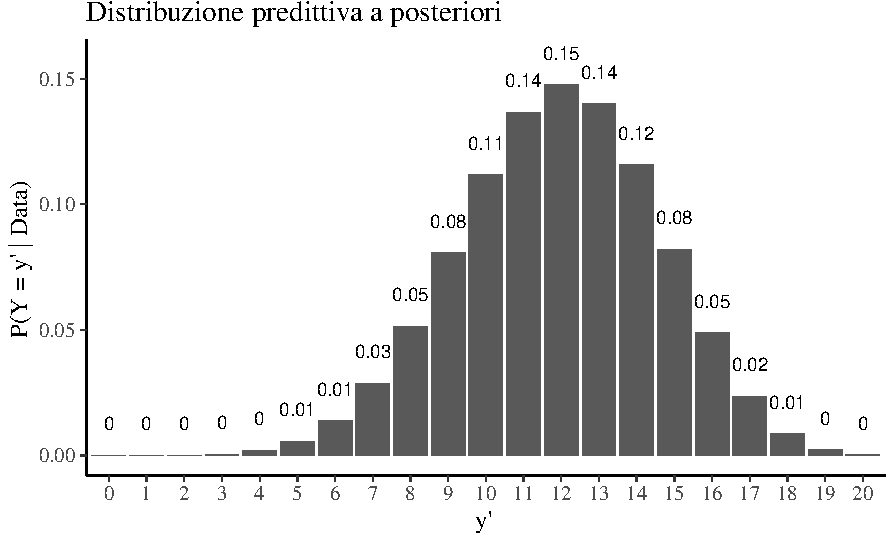
\includegraphics[width=0.8\linewidth]{046_ppc_files/figure-latex/unnamed-chunk-5-1} \end{center}

\noindent
È facile vedere che, in questo esempio, la distribuzione predittiva a posteriori \(p(\tilde{y} \mid y)\) è diversa dalla binomiale di parametro \(\theta = 23/30\):

\begin{Shaded}
\begin{Highlighting}[]
\FunctionTok{tibble}\NormalTok{(}
  \AttributeTok{heads =} \DecValTok{0}\SpecialCharTok{:}\DecValTok{20}\NormalTok{, }
  \AttributeTok{pmf =} \FunctionTok{dbinom}\NormalTok{(}\AttributeTok{x =} \DecValTok{0}\SpecialCharTok{:}\DecValTok{20}\NormalTok{, }\AttributeTok{size =} \DecValTok{20}\NormalTok{, }\AttributeTok{prob =} \DecValTok{23}\SpecialCharTok{/}\DecValTok{30}\NormalTok{)}
\NormalTok{) }\SpecialCharTok{\%\textgreater{}\%}
\FunctionTok{ggplot}\NormalTok{(}\FunctionTok{aes}\NormalTok{(}\AttributeTok{x =} \FunctionTok{factor}\NormalTok{(heads), }\AttributeTok{y =}\NormalTok{ pmf)) }\SpecialCharTok{+}
  \FunctionTok{geom\_col}\NormalTok{() }\SpecialCharTok{+}
  \FunctionTok{geom\_text}\NormalTok{(}
    \FunctionTok{aes}\NormalTok{(}\AttributeTok{label =} \FunctionTok{round}\NormalTok{(pmf, }\DecValTok{2}\NormalTok{), }\AttributeTok{y =}\NormalTok{ pmf }\SpecialCharTok{+} \FloatTok{0.01}\NormalTok{),}
    \AttributeTok{position =} \FunctionTok{position\_dodge}\NormalTok{(}\FloatTok{0.9}\NormalTok{),}
    \AttributeTok{size =} \DecValTok{3}\NormalTok{,}
    \AttributeTok{vjust =} \DecValTok{0}
\NormalTok{  ) }\SpecialCharTok{+}
  \FunctionTok{labs}\NormalTok{(}\AttributeTok{title =} \StringTok{"p(y | theta = 0.77)"}\NormalTok{,}
       \AttributeTok{x =} \StringTok{"y"}\NormalTok{,}
       \AttributeTok{y =} \StringTok{"Probabilità"}\NormalTok{) }
\end{Highlighting}
\end{Shaded}

\begin{center}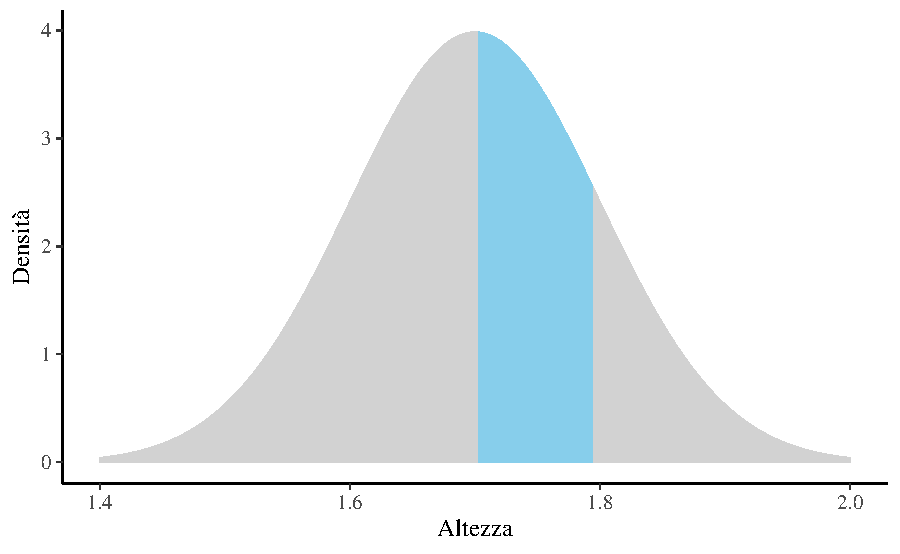
\includegraphics[width=0.8\linewidth]{046_ppc_files/figure-latex/unnamed-chunk-6-1} \end{center}

\noindent
In particolare, la \(p(\tilde{y} \mid y)\) ha una varianza maggiore di \(\Bin(y \mid \theta = 0.77, n = 20)\). Questa maggiore varianza riflette le due fonti di incertezza che sono presenti nella \eqref{eq:dist-pred-post}: l'incertezza sul valore del parametro (descritta dalla distribuzione a posteriori) e l'incertezza dovuta alla variabilità campionaria (descritta dalla funzione di verosimiglianza).
Possiamo concludere la discussione di questo esempio dicendo che, nel caso di 20 nuovi pazienti clinici, ci aspettiamo di osservare 12 pazienti che manifestano una depressione severa, anche se è ragionevole aspettarci un numero compreso, diciamo, tra 8 e 16.

Una volta trovata la distribuzione predittiva a posteriori \(p(\tilde{y} \mid y)\) diventa possibile rispondere a domande come: qual è la probabilità che almeno 10 dei 20 pazienti futuri mostrino una depressione grave? Rispondere a domande di questo tipo è possibile, ma richiede un po' di lavoro --- non ci sono funzioni \(\R\) che svolgano questi calcoli per noi. Tuttavia, non è importante imparare a risolvere problemi di questo tipo perché, in generale, anche per problemi solo leggermente più complessi di quello discusso qui, non sono disponibili espressioni analitiche della distribuzione predittiva a posteriori. Invece, è possibile trovare una approssimazione numerica della \(p(\tilde{y} \mid y)\) mediante simulazioni MCMC. Mediante un tale metodo è più facile rispondere a domande simili a quelle che ci siamo posti in questo Paragrafo.

\hypertarget{metodi-mcmc-per-la-distribuzione-predittiva-a-posteriori}{%
\section{Metodi MCMC per la distribuzione predittiva a posteriori}\label{metodi-mcmc-per-la-distribuzione-predittiva-a-posteriori}}

Se svolgiamo l'analisi bayesiana con il metodo MCMC, le repliche \(p(y^{rep} \mid y)\) (ovvero le stime delle possibili osservazioni future \(p(\tilde{y} \mid y)\)) possono essere ottenute nel modo seguente:

\begin{itemize}
\tightlist
\item
  campionare \(\theta_i \sim p(\theta \mid y)\), ovvero campionare un valore del parametro dalla distribuzione a posteriori;
\item
  campionare \(y^{rep} \sim p(y^{rep} \mid \theta_i)\), ovvero campionare il valore di un'osservazione dalla funzione di verosimiglianza condizionata al valore del parametro definito nel passo precedente.
\end{itemize}

\noindent
Se i due passaggi descritti sopra vengono ripetuti un numero sufficiente di volte, l'istogramma risultante approssimerà la distribuzione predittiva a posteriori che, in teoria (ma non in pratica) potrebbe essere ottenuta per via analitica (si veda il Paragrafo \ref{schema-beta-bin-distr-pred-post}).

Per fare un esempio concreto, esaminiamo il codice Stan che può essere usato per simulare \(p(y^{rep} \mid y)\). Consideriamo il caso semplice dell'inferenza su una proporzione --- si veda il Capitolo \ref{mod-binom}:

\begin{Shaded}
\begin{Highlighting}[]
\NormalTok{modelString }\OtherTok{=} \StringTok{"}
\StringTok{data \{}
\StringTok{  int\textless{}lower=0\textgreater{} N;}
\StringTok{  int\textless{}lower=0, upper=1\textgreater{} y[N];}
\StringTok{\}}
\StringTok{parameters \{}
\StringTok{  real\textless{}lower=0, upper=1\textgreater{} theta;}
\StringTok{\}}
\StringTok{model \{}
\StringTok{  theta \textasciitilde{} beta(2, 10);}
\StringTok{  y \textasciitilde{} bernoulli(theta);}
\StringTok{\}}
\StringTok{generated quantities \{}
\StringTok{  int y\_rep[N];}
\StringTok{  real log\_lik[N];}
\StringTok{  for (n in 1:N) \{}
\StringTok{    y\_rep[n] = bernoulli\_rng(theta);}
\StringTok{    log\_lik[n] = bernoulli\_lpmf(y[n] | theta);}
\StringTok{  \}}
\StringTok{\}}
\StringTok{"}
\FunctionTok{writeLines}\NormalTok{(modelString, }\AttributeTok{con =} \StringTok{"code/betabin23{-}30{-}2{-}10.stan"}\NormalTok{)}
\end{Highlighting}
\end{Shaded}

\noindent
Si noti che nel nel blocco \texttt{generated\ quantities} sono state aggiunte le istruzioni necessarie per simulare \(y^{rep}\), ovvero, \texttt{y\_rep{[}n{]}\ =\ bernoulli\_rng(theta)}. I dati dell'esempio sono:

\begin{Shaded}
\begin{Highlighting}[]
\NormalTok{data\_list }\OtherTok{\textless{}{-}} \FunctionTok{list}\NormalTok{(}
  \AttributeTok{N =} \DecValTok{30}\NormalTok{,}
  \AttributeTok{y =} \FunctionTok{c}\NormalTok{(}\FunctionTok{rep}\NormalTok{(}\DecValTok{1}\NormalTok{, }\DecValTok{23}\NormalTok{), }\FunctionTok{rep}\NormalTok{(}\DecValTok{0}\NormalTok{, }\DecValTok{7}\NormalTok{))}
\NormalTok{)}
\end{Highlighting}
\end{Shaded}

\noindent
Compiliamo il codice Stan

\begin{Shaded}
\begin{Highlighting}[]
\NormalTok{file }\OtherTok{\textless{}{-}} \FunctionTok{file.path}\NormalTok{(}\StringTok{"code"}\NormalTok{, }\StringTok{"betabin23{-}30{-}2{-}10.stan"}\NormalTok{)}
\NormalTok{mod }\OtherTok{\textless{}{-}} \FunctionTok{cmdstan\_model}\NormalTok{(file, }\AttributeTok{cpp\_options =} \FunctionTok{list}\NormalTok{(}\AttributeTok{stan\_opencl =} \ConstantTok{TRUE}\NormalTok{))}
\end{Highlighting}
\end{Shaded}

\noindent
ed eseguiamo il campionamento MCMC:

\begin{Shaded}
\begin{Highlighting}[]
\NormalTok{fit }\OtherTok{\textless{}{-}}\NormalTok{ mod}\SpecialCharTok{$}\FunctionTok{sample}\NormalTok{(}
  \AttributeTok{data =}\NormalTok{ data\_list,}
  \AttributeTok{iter\_sampling =}\NormalTok{ 4000L,}
  \AttributeTok{iter\_warmup =}\NormalTok{ 2000L,}
  \AttributeTok{seed =}\NormalTok{ SEED,}
  \AttributeTok{cores =}\NormalTok{ 4L,}
  \AttributeTok{chains =}\NormalTok{ 4L,}
  \AttributeTok{parallel\_chains =}\NormalTok{ 4L,}
  \AttributeTok{opencl\_ids =} \FunctionTok{c}\NormalTok{(}\DecValTok{0}\NormalTok{, }\DecValTok{0}\NormalTok{),}
  \AttributeTok{refresh =} \DecValTok{0}\NormalTok{,}
  \AttributeTok{thin =} \DecValTok{1}
\NormalTok{)}
\end{Highlighting}
\end{Shaded}

\noindent
Per comodità, trasformiamo l'oggetto \texttt{fit} in un oggetto di classe \texttt{stanfit}:

\begin{Shaded}
\begin{Highlighting}[]
\NormalTok{stanfit }\OtherTok{\textless{}{-}}\NormalTok{ rstan}\SpecialCharTok{::}\FunctionTok{read\_stan\_csv}\NormalTok{(fit}\SpecialCharTok{$}\FunctionTok{output\_files}\NormalTok{())}
\end{Highlighting}
\end{Shaded}

\noindent
Il contenuto dell'oggetto \texttt{stanfit} può essere esaminato nel modo seguente:

\begin{Shaded}
\begin{Highlighting}[]
\NormalTok{list\_of\_draws }\OtherTok{\textless{}{-}} \FunctionTok{extract}\NormalTok{(stanfit)}
\FunctionTok{print}\NormalTok{(}\FunctionTok{names}\NormalTok{(list\_of\_draws))}
\CommentTok{\#\textgreater{} [1] "theta"   "y\_rep"   "log\_lik" "lp\_\_"}
\end{Highlighting}
\end{Shaded}

\noindent 
Dall'oggetto \texttt{list\_of\_draws} recuperiamo \texttt{y\_rep}:

\begin{Shaded}
\begin{Highlighting}[]
\NormalTok{y\_bern }\OtherTok{\textless{}{-}}\NormalTok{ list\_of\_draws}\SpecialCharTok{$}\NormalTok{y\_rep}
\FunctionTok{dim}\NormalTok{(y\_bern)}
\CommentTok{\#\textgreater{} [1] 16000    30}
\FunctionTok{head}\NormalTok{(y\_bern)}
\CommentTok{\#\textgreater{}           }
\CommentTok{\#\textgreater{} iterations [,1] [,2] [,3] [,4] [,5] [,6] [,7] [,8] [,9] [,10] [,11] [,12] [,13]}
\CommentTok{\#\textgreater{}       [1,]    0    1    1    0    0    1    1    1    1     1     1     0     0}
\CommentTok{\#\textgreater{}       [2,]    1    0    1    0    1    1    1    1    1     1     1     1     1}
\CommentTok{\#\textgreater{}       [3,]    1    1    0    1    1    1    0    1    1     0     0     1     1}
\CommentTok{\#\textgreater{}       [4,]    0    1    1    1    0    1    1    1    1     1     1     1     0}
\CommentTok{\#\textgreater{}       [5,]    0    1    1    0    0    1    1    0    1     0     1     1     0}
\CommentTok{\#\textgreater{}       [6,]    1    1    1    0    0    0    0    1    0     1     1     1     1}
\CommentTok{\#\textgreater{}           }
\CommentTok{\#\textgreater{} iterations [,14] [,15] [,16] [,17] [,18] [,19] [,20] [,21] [,22] [,23] [,24]}
\CommentTok{\#\textgreater{}       [1,]     0     1     1     0     1     0     1     1     0     1     0}
\CommentTok{\#\textgreater{}       [2,]     1     0     1     0     0     1     1     1     0     1     1}
\CommentTok{\#\textgreater{}       [3,]     1     1     1     1     1     1     1     0     1     0     1}
\CommentTok{\#\textgreater{}       [4,]     1     0     0     1     1     1     1     1     1     1     1}
\CommentTok{\#\textgreater{}       [5,]     1     1     1     0     1     1     1     0     0     1     1}
\CommentTok{\#\textgreater{}       [6,]     0     1     1     0     0     1     0     0     1     0     1}
\CommentTok{\#\textgreater{}           }
\CommentTok{\#\textgreater{} iterations [,25] [,26] [,27] [,28] [,29] [,30]}
\CommentTok{\#\textgreater{}       [1,]     0     0     1     1     1     0}
\CommentTok{\#\textgreater{}       [2,]     1     1     0     1     1     1}
\CommentTok{\#\textgreater{}       [3,]     0     1     0     1     1     0}
\CommentTok{\#\textgreater{}       [4,]     1     0     0     1     0     1}
\CommentTok{\#\textgreater{}       [5,]     1     1     0     1     0     0}
\CommentTok{\#\textgreater{}       [6,]     1     1     1     1     1     0}
\end{Highlighting}
\end{Shaded}

\noindent
Dato che il codice Stan definisce un modello per i dati grezzi (ovvero, per ciascuna singola prova Bernoulliana del campione), ogni riga di \texttt{y\_bern} include 30 colonne, ciascuna delle quali corrisponde ad un campione (\(n\) = 16000 in questa simulazione) di possibili valori futuri \(y_i \in \{0, 1\}\). Per ottenere una stima della distribuzione predittiva a posteriori \texttt{p(y\_rep)}, ovvero, una stima della probabilità associata a ciascuno dei possibili numeri di ``successi'' in \(N = 30\) nuove prove future, è sufficiente calcolare la proporzione di valori 1 in ciascuna riga:

\begin{Shaded}
\begin{Highlighting}[]
\FunctionTok{data.frame}\NormalTok{(}\AttributeTok{y\_rep =} \FunctionTok{rowSums}\NormalTok{(y\_bern)) }\SpecialCharTok{\%\textgreater{}\%} 
  \FunctionTok{ggplot}\NormalTok{(}\FunctionTok{aes}\NormalTok{(}\AttributeTok{x =}\NormalTok{ y\_rep, }\FunctionTok{after\_stat}\NormalTok{(density))) }\SpecialCharTok{+} 
  \FunctionTok{geom\_histogram}\NormalTok{(}\AttributeTok{binwidth =} \DecValTok{1}\NormalTok{) }
\end{Highlighting}
\end{Shaded}

\begin{center}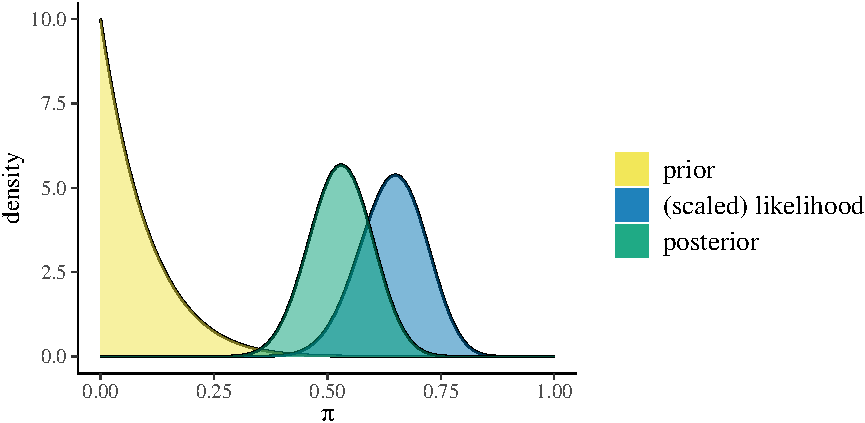
\includegraphics[width=0.8\linewidth]{046_ppc_files/figure-latex/unnamed-chunk-14-1} \end{center}

\hypertarget{posterior-predictive-checks}{%
\section{Posterior predictive checks}\label{posterior-predictive-checks}}

La distribuzione predittiva a posteriori viene utilizzata per eseguire i cosiddetti \emph{controlli predittivi a posteriori} (\emph{Posterior Predictive Checks}, PPC). Ricordiamo che la distribuzione predittiva a posteriori corrisponde alla simulazione di un campione di dati generati utilizzando le proprietà del modello adattato. Nei PPC si realizza un confronto grafico tra \(p(y^{rep} \mid y)\) e i dati osservati \(y\).
Confrontando visivamente gli aspetti chiave dei dati previsti futuri \(y^{rep}\) e dei dati osservati \(y\) possiamo determinare se il modello è adeguato.

Oltre al confronto tra le distribuzioni \(p(y)\) e \(p(y^{rep})\) è anche possibile un confronto tra la distribuzione di varie statistiche descrittive, i cui valori sono calcolati su diversi campioni \(y^{rep}\), e le corrispondenti statistiche descrittive calcolate sui dati osservati. Vengono solitamente considerate statistiche descrittive quali la media, la varianza, la deviazione standard, il minimo o il massimo. Ma confronti di questo tipo sono possibili per qualunque statistica descrittiva. Questi confronti sono chiamati PPC.

\hypertarget{ppc-per-la-velocituxe0-della-luce}{%
\subsection{PPC per la velocità della luce}\label{ppc-per-la-velocituxe0-della-luce}}

Qui di seguito esamineremo un set di dati che non seguono la distribuzione normale \autocite{gelman2020regression}. I dati corrispondono ad una serie di misurazioni prese da Simon Newcomb nel 1882 come parte di un esperimento per stimare la velocità della luce. A questi dati verrà (inappropriatamente) adattata una distribuzione normale. L'obiettivo dell'esempio è quello di mostrare come i PPC possono rivelare la mancanza di adattamento di un modello ai dati.

\begin{Shaded}
\begin{Highlighting}[]
\FunctionTok{library}\NormalTok{(}\StringTok{"MASS"}\NormalTok{)}
\FunctionTok{data}\NormalTok{(}\StringTok{"newcomb"}\NormalTok{)}
\FunctionTok{hist}\NormalTok{(newcomb)}
\end{Highlighting}
\end{Shaded}

\begin{center}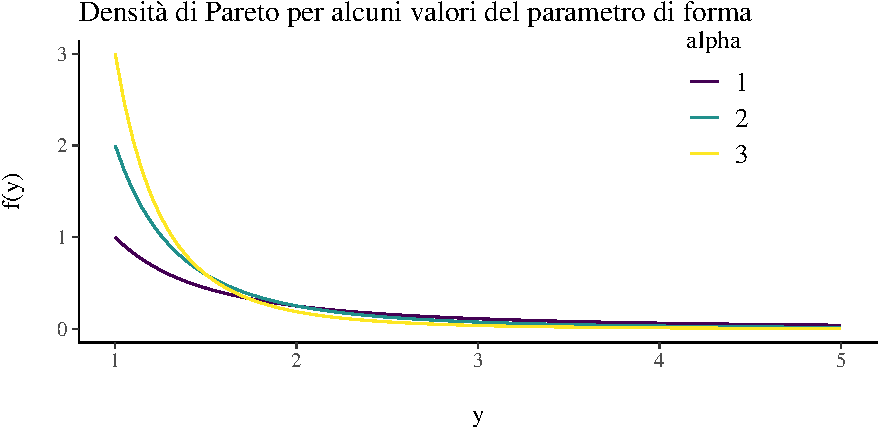
\includegraphics[width=0.8\linewidth]{046_ppc_files/figure-latex/unnamed-chunk-15-1} \end{center}

\noindent
Creiamo un oggetto di tipo \texttt{list} dove inserire i dati:

\begin{Shaded}
\begin{Highlighting}[]
\NormalTok{data\_list }\OtherTok{\textless{}{-}} \FunctionTok{list}\NormalTok{(}
  \AttributeTok{y =}\NormalTok{ newcomb,}
  \AttributeTok{N =} \FunctionTok{length}\NormalTok{(newcomb)}
\NormalTok{)}
\end{Highlighting}
\end{Shaded}

\noindent
Il codice Stan per il modello normale è il seguente:

\begin{Shaded}
\begin{Highlighting}[]
\NormalTok{modelString }\OtherTok{\textless{}{-}} \StringTok{"}
\StringTok{data \{}
\StringTok{  int\textless{}lower=0\textgreater{} N;}
\StringTok{  vector[N] y;}
\StringTok{\}}
\StringTok{parameters \{}
\StringTok{  real mu;}
\StringTok{  real\textless{}lower=0\textgreater{} sigma;}
\StringTok{\}}
\StringTok{model \{}
\StringTok{  mu \textasciitilde{} normal(25, 10);}
\StringTok{  sigma \textasciitilde{} cauchy(0, 10);}
\StringTok{  y \textasciitilde{} normal(mu, sigma);}
\StringTok{\}}
\StringTok{generated quantities \{}
\StringTok{  vector[N] y\_rep;}
\StringTok{  for (n in 1:N) \{}
\StringTok{    y\_rep[n] = normal\_rng(mu, sigma);}
\StringTok{  \}}
\StringTok{\}}
\StringTok{"}
\FunctionTok{writeLines}\NormalTok{(modelString, }\AttributeTok{con =} \StringTok{"code/newcomb.stan"}\NormalTok{)}
\end{Highlighting}
\end{Shaded}

\noindent
Adattiamo il modello ai dati

\begin{Shaded}
\begin{Highlighting}[]
\NormalTok{file }\OtherTok{\textless{}{-}} \FunctionTok{file.path}\NormalTok{(}\StringTok{"code"}\NormalTok{, }\StringTok{"newcomb.stan"}\NormalTok{)}
\NormalTok{mod }\OtherTok{\textless{}{-}} \FunctionTok{cmdstan\_model}\NormalTok{(file)}
\NormalTok{fit }\OtherTok{\textless{}{-}}\NormalTok{ mod}\SpecialCharTok{$}\FunctionTok{sample}\NormalTok{(}
  \AttributeTok{data =}\NormalTok{ data\_list,}
  \AttributeTok{iter\_sampling =}\NormalTok{ 4000L,}
  \AttributeTok{iter\_warmup =}\NormalTok{ 2000L,}
  \AttributeTok{seed =}\NormalTok{ SEED,}
  \AttributeTok{chains =}\NormalTok{ 4L,}
  \AttributeTok{cores =}\NormalTok{ 4L,}
  \AttributeTok{refresh =} \DecValTok{0}\NormalTok{,}
  \AttributeTok{thin =} \DecValTok{1}
\NormalTok{)}
\end{Highlighting}
\end{Shaded}

\noindent
e otteniamo le seguenti stime dei parametri \(\mu\) e \(\sigma\):

\begin{Shaded}
\begin{Highlighting}[]
\NormalTok{fit}\SpecialCharTok{$}\FunctionTok{summary}\NormalTok{(}\FunctionTok{c}\NormalTok{(}\StringTok{"mu"}\NormalTok{, }\StringTok{"sigma"}\NormalTok{))}
\CommentTok{\#\textgreater{} \# A tibble: 2 x 10}
\CommentTok{\#\textgreater{}   variable  mean median    sd   mad    q5   q95  rhat ess\_bulk ess\_tail}
\CommentTok{\#\textgreater{}   \textless{}chr\textgreater{}    \textless{}dbl\textgreater{}  \textless{}dbl\textgreater{} \textless{}dbl\textgreater{} \textless{}dbl\textgreater{} \textless{}dbl\textgreater{} \textless{}dbl\textgreater{} \textless{}dbl\textgreater{}    \textless{}dbl\textgreater{}    \textless{}dbl\textgreater{}}
\CommentTok{\#\textgreater{} 1 mu        26.2   26.2 1.33  1.32  24.0   28.4  1.00   12233.    9822.}
\CommentTok{\#\textgreater{} 2 sigma     10.9   10.8 0.973 0.953  9.39  12.6  1.00   12499.   10060.}
\end{Highlighting}
\end{Shaded}

\noindent
Trasformiamo \texttt{fit} in un oggetto \texttt{stanfit}:

\begin{Shaded}
\begin{Highlighting}[]
\NormalTok{stanfit }\OtherTok{\textless{}{-}}\NormalTok{ rstan}\SpecialCharTok{::}\FunctionTok{read\_stan\_csv}\NormalTok{(fit}\SpecialCharTok{$}\FunctionTok{output\_files}\NormalTok{())}
\end{Highlighting}
\end{Shaded}

\noindent
La distribuzione a posteriori di \(\mu\) è

\begin{Shaded}
\begin{Highlighting}[]
\NormalTok{mu\_draws }\OtherTok{\textless{}{-}} \FunctionTok{as.matrix}\NormalTok{(stanfit, }\AttributeTok{pars =} \StringTok{"mu"}\NormalTok{)}
\FunctionTok{mcmc\_areas}\NormalTok{(mu\_draws, }\AttributeTok{prob =} \FloatTok{0.95}\NormalTok{) }\CommentTok{\# color 95\% interval}
\end{Highlighting}
\end{Shaded}

\begin{center}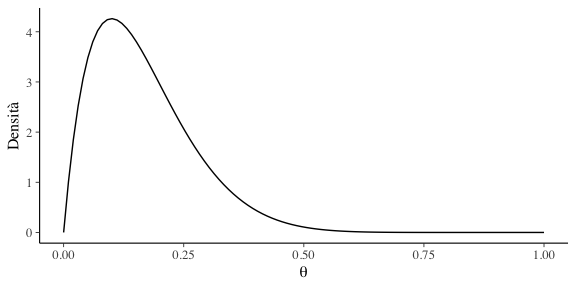
\includegraphics[width=0.8\linewidth]{046_ppc_files/figure-latex/unnamed-chunk-21-1} \end{center}

\noindent
Confrontiamo \(\mu\) con la media di \(y\):

\begin{Shaded}
\begin{Highlighting}[]
\FunctionTok{mean}\NormalTok{(newcomb)}
\CommentTok{\#\textgreater{} [1] 26.2}
\end{Highlighting}
\end{Shaded}

\noindent
Anche se trova la media giusta, il modello non è comunque adeguato a prevedere le altre proprietà della \(y\). Estraiamo \(y^{rep}\) dall'oggetto \texttt{stanfit}:

\begin{Shaded}
\begin{Highlighting}[]
\NormalTok{y\_rep }\OtherTok{\textless{}{-}} \FunctionTok{as.matrix}\NormalTok{(stanfit, }\AttributeTok{pars =} \StringTok{"y\_rep"}\NormalTok{)}
\FunctionTok{dim}\NormalTok{(y\_rep) }
\CommentTok{\#\textgreater{} [1] 16000    66}
\end{Highlighting}
\end{Shaded}

\noindent
I valori \texttt{y\_rep} sono i dati della distribuzione predittiva a posteriori che sono stati simulati usando gli stessi valori \(X\) dei predittori utilizzati per adattare il modello. Il confronto tra l'istogramma della \(y\) e gli istogrammi di diversi campioni \(y^{rep}\) mostra una scarsa corrispondenza tra i due:

\begin{Shaded}
\begin{Highlighting}[]
\FunctionTok{ppc\_hist}\NormalTok{(data\_list}\SpecialCharTok{$}\NormalTok{y, y\_rep[}\DecValTok{1}\SpecialCharTok{:}\DecValTok{8}\NormalTok{, ], }\AttributeTok{binwidth =} \DecValTok{1}\NormalTok{)}
\end{Highlighting}
\end{Shaded}

\begin{center}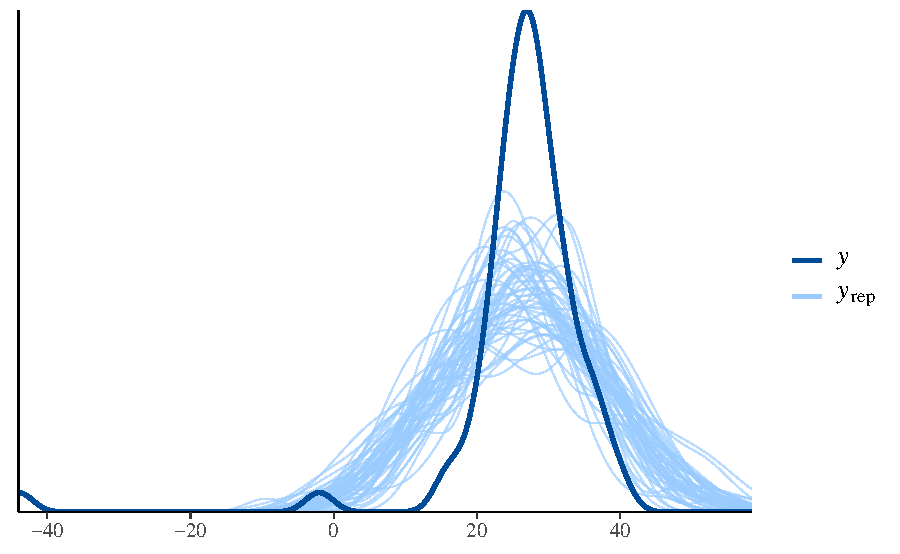
\includegraphics[width=0.8\linewidth]{046_ppc_files/figure-latex/unnamed-chunk-24-1} \end{center}

\noindent
Alla stessa conclusione si giunge tramite un confronto tra la funzione di densità empirica della \(y\) e quella di diversi campioni \(y^{rep}\):

\begin{Shaded}
\begin{Highlighting}[]
\FunctionTok{ppc\_dens\_overlay}\NormalTok{(data\_list}\SpecialCharTok{$}\NormalTok{y, y\_rep[}\DecValTok{1}\SpecialCharTok{:}\DecValTok{50}\NormalTok{, ])}
\end{Highlighting}
\end{Shaded}

\begin{center}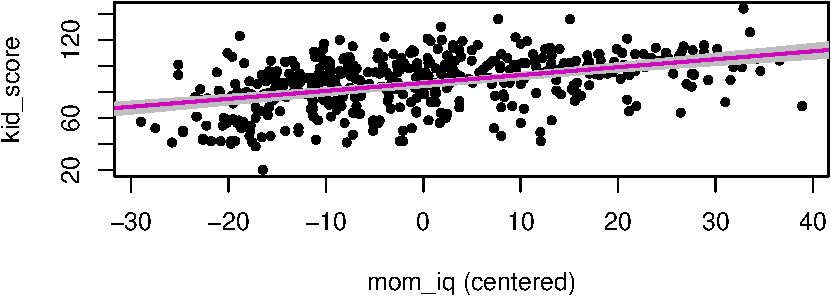
\includegraphics[width=0.8\linewidth]{046_ppc_files/figure-latex/unnamed-chunk-25-1} \end{center}

\noindent
Generiamo ora i PPC per la media e il minimo della distribuzione:

\begin{Shaded}
\begin{Highlighting}[]
\FunctionTok{ppc\_stat\_2d}\NormalTok{(data\_list}\SpecialCharTok{$}\NormalTok{y, y\_rep, }\AttributeTok{stat =} \FunctionTok{c}\NormalTok{(}\StringTok{"mean"}\NormalTok{, }\StringTok{"min"}\NormalTok{))}
\end{Highlighting}
\end{Shaded}

\begin{center}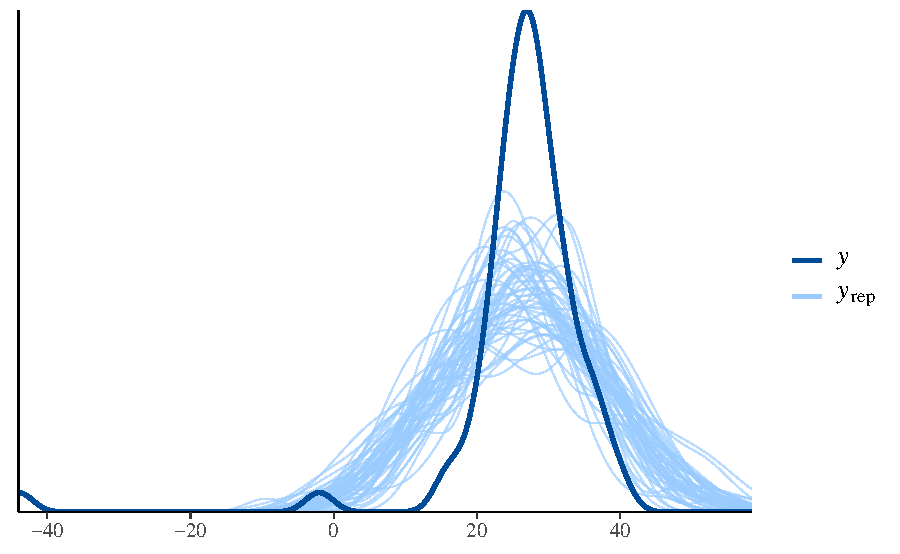
\includegraphics[width=0.8\linewidth]{046_ppc_files/figure-latex/unnamed-chunk-26-1} \end{center}

\noindent
Mentre la media viene riprodotta accuratamente dal modello (come abbiamo visto sopra), ciò non è vero per il minimo dela distribuzione. L'origine di questa mancanza di adattamento è il fatto che la distribuzione delle misurazioni della velocità della luce è asimmetrica negativa. Dato che ci sono poche osservazioni nella coda negativa della distribuzione, solo per fare un esempio, utilizzeremo ora un secondo modello che ipotizza una distribuzione \(t\) di Student:

\begin{Shaded}
\begin{Highlighting}[]
\NormalTok{modelString }\OtherTok{=} \StringTok{"}
\StringTok{data \{}
\StringTok{  int\textless{}lower=0\textgreater{} N;}
\StringTok{  vector[N] y;}
\StringTok{\}}
\StringTok{parameters \{}
\StringTok{  real mu;}
\StringTok{  real\textless{}lower=0\textgreater{} sigma;}
\StringTok{  real\textless{}lower=0\textgreater{} nu;}
\StringTok{\}}
\StringTok{model \{}
\StringTok{  mu \textasciitilde{} normal(25, 10);}
\StringTok{  sigma \textasciitilde{} cauchy(0, 10);}
\StringTok{  nu \textasciitilde{} cauchy(0, 10);}
\StringTok{  y \textasciitilde{} student\_t(nu, mu, sigma);}
\StringTok{\}}
\StringTok{generated quantities \{}
\StringTok{  vector[N] y\_rep;}
\StringTok{  for (n in 1:N) \{}
\StringTok{    y\_rep[n] = student\_t\_rng(nu, mu, sigma);}
\StringTok{  \}}
\StringTok{\}}
\StringTok{"}
\FunctionTok{writeLines}\NormalTok{(modelString, }\AttributeTok{con =} \StringTok{"code/newcomb2.stan"}\NormalTok{)}
\end{Highlighting}
\end{Shaded}

\noindent
Adattiamo questo secondo modello ai dati.

\begin{Shaded}
\begin{Highlighting}[]
\NormalTok{file }\OtherTok{\textless{}{-}} \FunctionTok{file.path}\NormalTok{(}\StringTok{"code"}\NormalTok{, }\StringTok{"newcomb2.stan"}\NormalTok{)}
\NormalTok{mod }\OtherTok{\textless{}{-}} \FunctionTok{cmdstan\_model}\NormalTok{(file)}
\NormalTok{fit }\OtherTok{\textless{}{-}}\NormalTok{ mod}\SpecialCharTok{$}\FunctionTok{sample}\NormalTok{(}
  \AttributeTok{data =}\NormalTok{ data\_list,}
  \AttributeTok{iter\_sampling =}\NormalTok{ 4000L,}
  \AttributeTok{iter\_warmup =}\NormalTok{ 2000L,}
  \AttributeTok{seed =}\NormalTok{ SEED,}
  \AttributeTok{chains =}\NormalTok{ 4L,}
  \AttributeTok{cores =}\NormalTok{ 4L,}
  \AttributeTok{parallel\_chains =}\NormalTok{ 2L,}
  \AttributeTok{refresh =} \DecValTok{0}\NormalTok{,}
  \AttributeTok{thin =} \DecValTok{1}
\NormalTok{)}
\CommentTok{\#\textgreater{} Running MCMC with 4 parallel chains...}
\CommentTok{\#\textgreater{} }
\CommentTok{\#\textgreater{} Chain 1 finished in 0.3 seconds.}
\CommentTok{\#\textgreater{} Chain 2 finished in 0.3 seconds.}
\CommentTok{\#\textgreater{} Chain 3 finished in 0.3 seconds.}
\CommentTok{\#\textgreater{} Chain 4 finished in 0.3 seconds.}
\CommentTok{\#\textgreater{} }
\CommentTok{\#\textgreater{} All 4 chains finished successfully.}
\CommentTok{\#\textgreater{} Mean chain execution time: 0.3 seconds.}
\CommentTok{\#\textgreater{} Total execution time: 0.4 seconds.}
\end{Highlighting}
\end{Shaded}

\noindent
Per questo secondo modello il confronto tra la funzione di densità empirica della \(y\) e quella di diversi campioni \(y^{rep}\) risulta adeguato:

\begin{Shaded}
\begin{Highlighting}[]
\NormalTok{stanfit }\OtherTok{\textless{}{-}}\NormalTok{ rstan}\SpecialCharTok{::}\FunctionTok{read\_stan\_csv}\NormalTok{(fit}\SpecialCharTok{$}\FunctionTok{output\_files}\NormalTok{())}
\NormalTok{y\_rep }\OtherTok{\textless{}{-}} \FunctionTok{as.matrix}\NormalTok{(stanfit, }\AttributeTok{pars =} \StringTok{"y\_rep"}\NormalTok{)}
\FunctionTok{ppc\_dens\_overlay}\NormalTok{(data\_list}\SpecialCharTok{$}\NormalTok{y, y\_rep[}\DecValTok{1}\SpecialCharTok{:}\DecValTok{50}\NormalTok{, ])}
\end{Highlighting}
\end{Shaded}

\begin{center}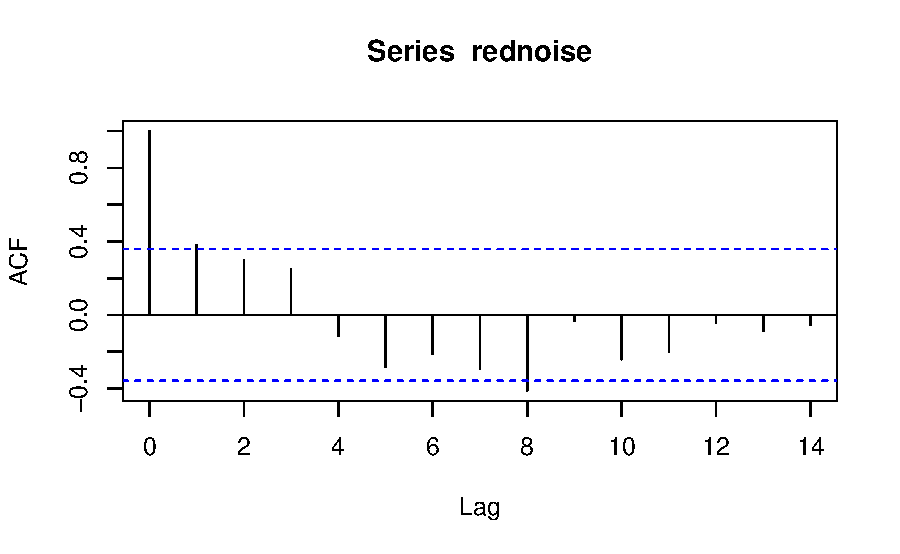
\includegraphics[width=0.8\linewidth]{046_ppc_files/figure-latex/unnamed-chunk-29-1} \end{center}

\noindent
Inoltre, anche la statistica ``minimo della distribuzione'' viene ben predetta dal modello.

\begin{Shaded}
\begin{Highlighting}[]
\FunctionTok{ppc\_stat\_2d}\NormalTok{(data\_list}\SpecialCharTok{$}\NormalTok{y, y\_rep, }\AttributeTok{stat =} \FunctionTok{c}\NormalTok{(}\StringTok{"mean"}\NormalTok{, }\StringTok{"min"}\NormalTok{))}
\end{Highlighting}
\end{Shaded}

\begin{center}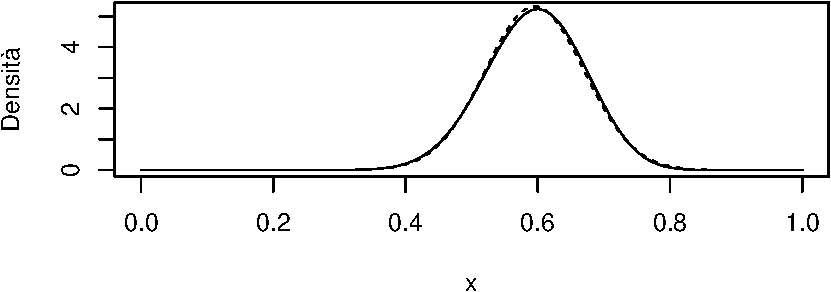
\includegraphics[width=0.8\linewidth]{046_ppc_files/figure-latex/unnamed-chunk-30-1} \end{center}

\noindent
In conclusione, per le misurazioni della velocità della luce di Newcomb l'accuratezza predittiva del modello basato sulla distribuzione \(t\) di Student è chiaramente migliore di quella del modello normale.

\hypertarget{considerazioni-conclusive}{%
\section*{Considerazioni conclusive}\label{considerazioni-conclusive}}
\addcontentsline{toc}{section}{Considerazioni conclusive}

Questo capitolo presenta i controlli predittivi a posteriori. A questo proposito è necessario notare un punto importante: i controlli predittivi a posteriori, quando suggeriscono un buon adattamento del modello alle caratterische dei dati previsti futuri \(y^{rep}\), non forniscono necessariamente una forte evidenza della capacità del modello di generalizzarsi a nuovi campioni di dati. Una tale evidenza sulla generalizzabilità del modello può solo essere fornita da studi di \emph{holdout validation}, ovvero da studi nei quali viene utilizzato un \emph{nuovo} campione di dati. Se i PPC mostrano un cattivo adattamento del modello ai dati previsti futuri, però, questo controllo fornisce una forte evidenza di una errata specificazione del modello.


% Bibliography
%%%%%%%%%%%%%%%%%%%%%%%%%%%%%%%%%%%%%%%%%%%%%%%%%%%%%%%%%%

\backmatter
\SmallMargins

\printbibliography
\onecolumn


% Tables (of tables, of figures)
%%%%%%%%%%%%%%%%%%%%%%%%%%%%%%%%%%%%%%%%%%%%%%%%%%%%%%%%%%


\cleardoublepage
\LargeMargins
\listoffigures


% After-body (LaTeX code inclusion)
%%%%%%%%%%%%%%%%%%%%%%%%%%%%%%%%%%%%%%%%%%%%%%%%%%%%%%%%%%




% Back cover
%%%%%%%%%%%%%%%%%%%%%%%%%%%%%%%%%%%%%%%%%%%%%%%%%%%%%%%%%%%

% Even page, small margins, no running head, no page number.
\evenpage
\SmallMargins
\thispagestyle{empty}

\begin{normalsize}

\begin{description}

\selectlanguage{italian}
\item[Abstract]
This document contains the material of the lessons of Psicometria B000286 (2021/2022) aimed at students of the first year of the Degree Course in Psychological Sciences and Techniques of the University of Florence, Italy.
\item[Keywords]
Data science, Bayesian statistics.
~\\

\end{description}

\end{normalsize}


\end{document}
